\documentclass{article}
\usepackage[utf8]{inputenc}
\usepackage{subfig}

%References
\usepackage{natbib}
%IMPORTANT use https://www.citationmachine.net/ if you need to generate references!
% \citep{reference} creates Harvard Style references throughout

%Colors
\usepackage{xcolor}

\usepackage[protrusion=true,expansion]{microtype}

%Code Markup
\usepackage[outputdir=cache]{minted}
%Syntax Highlighting Style
\definecolor{bggray}{RGB}{40,40,40}
\newmintedfile[javacode]{java}{
	style=fruity,
	bgcolor=bggray,
	linenos,
	breaklines,
	tabsize=2,
	obeytabs
}

\newmintedfile[bashoutput]{text} {
	style=fruity,
	bgcolor=bggray,
	breaklines,
	tabsize =2,
	obeytabs
}

\newmintedfile[armfile]{ARM} {
	style=fruity,
	bgcolor=bggray,
	breaklines,
	tabsize =2,
	obeytabs
}

%Page Margins and stuff
\usepackage{geometry}
 \geometry{
 a4paper,
 total={170mm,257mm},
 left=20mm,
 }

%Pictures
\usepackage{graphicx}
\graphicspath{ {./images/} }

%Move the title position
\usepackage{titling}

\setlength{\droptitle}{-8.5em} %Up, near the top but not too high

\title{Assignment 4 - CT2109 Object Oriented Programming: Data Structures and Algorithms}
\author{Daniel Hannon (19484286)}
\date{April 2021}

\begin{document}
	\maketitle
	\section{Overview}
	The aim of this report is to give an Overview/Definition and example of:
	\begin{itemize}
		\item Polynomial Problems
		\item Non-Deterministic Polynomial Problems
		\item NP-Hard Problems
		\item NP-Complete Problems
	\end{itemize}
	And an introduction to the P versus NP problem along with some background and the reprecussions of the result when it is inevitably reached.
	\section{Polynomial Problems}
	\subsection{Outline of a Polynomial Problem}
	A Polynomial Problem is that can be solved by a Deterministic algorithm in Polynomial time. A Deterministic algorithm is an algorithm that always reproduces the exact same results given the exact same inputs by performing the exact same steps. As a result problems in P can be defined as "Tractable" where a tractable problem is one that can be solved in reasonable time. They can essentially be boiled down to $$O(p(n))$$ where \textit{p(n)} denotes a Polynomial algortihm to calculate the time to solve it.
	\subsection{Example of a Polynomial Problem}
	A fairly straightforward example of a Polynomial Problem is the Karatsuba algorithm for multiplying two large numbers, it has an approximated complexity of: $$O({n}^{1.585})$$ and it is a proven more efficient method of multiplying two numbers than the classic schoolbook method it can be performed recursively.\citep{weiss_2006} It can be done in the following way:
	\begin{enumerate}
		\item Check if either number is less than 10, if yes return the product of both numbers.
		\item Get the highest shared whole-number log10 value between the two numbers.
		\item Record the value from step 2 divide it by two and round down.
		\item Split the numbers at this log of 10 into the form $leading\_digits * {10}^{step2\_value} + following\_digits$
		\item Start from step 1 again with the following\_digits values from both numbers and record this result
		\item Start from step 1 again with $leading\_digits + following\_digits$ for either value and record this result
		\item Start from step 1 with the leading digits from step 4 for either number and record the result
		\item Return $$(s\_7\_res * {10}^{(s\_3\_res * 2)}) + ((s\_6\_res - s\_7\_res - s\_5\_res) * {10}^{s\_3\_res})) + s\_5\_res$$ where the form s\_x\_res denotes result from step x
	\end{enumerate}
	As it follows a Deterministic algorithm to achieve a result and it is tractable it belongs to class P.
	\section{Non-Deterministic Polynomial Problems}
	\subsection{Outline of a Non-Deterministic Polynomial Problem}
		A Non-Deterministic Polynomial problem is one that uses a Non-Deterministic Algorithm as a means to generate a potential solution, either randomly, or systematically, then it verifies whether it is true or not and repeats ad-infinitum unless it finds a solution.\\
		If the verification step is Polynomial then the algorithm and by extension, the problem belong to NP. This of course implies that P is a subset of NP as anything that can be solved in Polynomial time can by definition be verified in Polynomial time.
	\subsection{Example of a Non-Deterministic Polynomial Problem}
	Although very often frowned upon, cracking a password by means of a brute force would constitute as an NP problem as it uses some form of algorithm to generate a potential password and then it is checked against the password and whether or not it is the password can be verified in Polynomial time.\citep{atkins-bittner_2014}
	\section{NP-Complete Problems}
		\subsection{Outline of an NP-Complete Problem}
			An NP-Complete Problem is a problem that is as at minimum, as hard as all other problems in NP. These algorithms are comparatible to others in NP but not necessecarily reducible to problems in P (this will be explored later on).\\
			All NP-Complete problems can be solved by means of a bruteforce algorithm. All NP-Complete problems are also Polynominally Reduceable which means there exists some Polynomial-time transformation to convert inputs of one to those of another algorithm that's NP-Complete.
		\subsection{Example of an NP-Complete Problem}
			\begin{figure}[H]
				\centering
				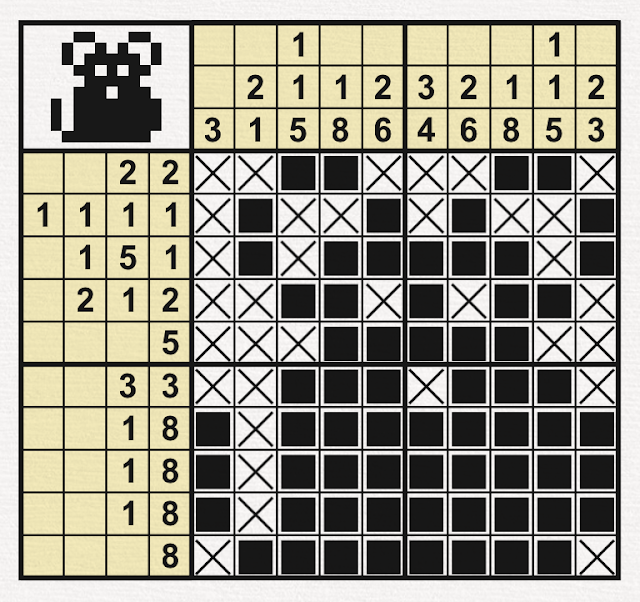
\includegraphics[width=0.25\textwidth]{MOUSE.PNG}
				\caption{An Example of a Solved Nonogram\citep{10x10mouse_2016}}
				\end{figure}
				A good example of an NP-Complete problem is a nonogram. A nonogram is a japanese picture puzzle where you are presented with an m x n grid and a list of groupings of colored squares for each row/column. A Nonogram is in in NP as a solution is extremely easy to verify and can be done in Polynomial time but is currently not in P as there is currently no known algorithm to solve every nonogram in Polynomial time and thus requires a bruteforce search. It was proven to be NP-Complete by demonstrating that the already known to be NP-Complete 3-Dimension Matching Problem \citep{karp1972reducibility} could be reduced to a Nonogram and by extension the already known to be NP-Complete Another Solution Problem for 3 Dimensional Matching could be reduced to the Another Solution Problem for a Nonogram and consequently Nonograms are NP-Complete.\citep{ueda1996np}\\
	\section{NP-Hard Problems}
		\subsection{Outline of an NP-Hard Problem}
			An NP-Hard Problem is a problem that is at least as hard as an NP-Complete Problem, but unlike NP Problems, they do not need to be decision Problems which also means that some of them may be unsolvable by a computer. A further classification is that An algorithm H is NP-Hard if there is a when any problem L in NP-Complete can be solved by means of H in Polynomial-time \citep{10.1145_1008304.1008305}
			\subsection{Example of an NP-Hard Problem}
				\begin{figure}[H]
					\centering
					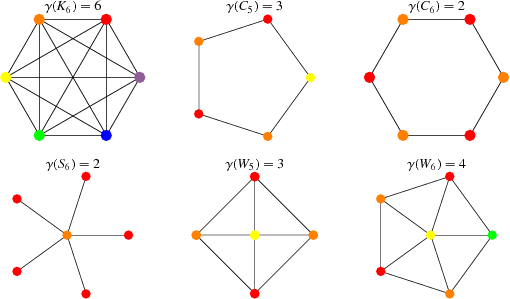
\includegraphics[width=0.35\textwidth]{chromatic_number.png}
					\caption{Examples of graphs and their chromatic numbers \cite{weisstein}}
				\end{figure}
				A very good example of an NP-Hard problem is that of the "Minimum-Color Problem" where you must calculate the chromatic number (Minimum number of Colors needed to ensure no two nodes of the same color are adjacent) of an undirected graph G.
	\section{The P versus NP Problem}
		\begin{figure}[H]
			\centering
			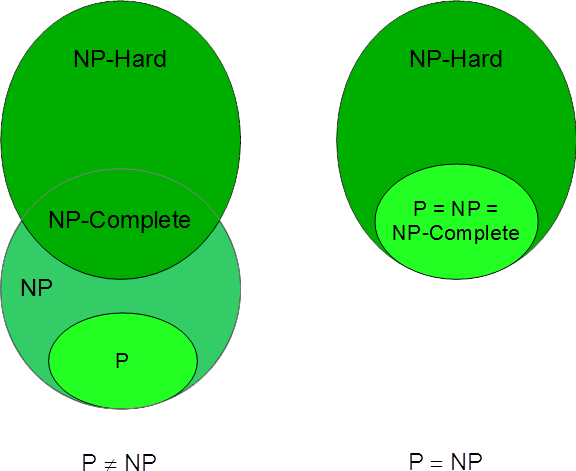
\includegraphics[width=0.3\textwidth]{p_np.png}
			\caption{Graph for if $P = NP$ and if $P \neq NP$ \citep{pnpimage}}
		\end{figure}
		\begin{quote}
		\centering
		\textit{"P = NP where N = 1" $\sim$Unknown}
		\end{quote}
	The P versus NP problem is one very important problem in all fields of Computer Science. It was first Introduced by Stephen Cook in 1973 when he published the paper "The complexity of theorem proving procedures" and in 2000 the Clay Mathematics Institute declared it as one of the seven "Millennium Prize Problems", each of these problems was at the time an unsolved problem in Mathematics, and if someone were to offer an accepted solution either proving, or disproving it, they would recieve \$1,000,000. Thusfar only one of these problems has been solved. In Essence the P versus NP problem poses the question that for any problem that can be quickly verified does there exist a means in which it can be quickly solved? Some academics such as Donald Knuth believe that P = NP but he stated the runtime of an algortihm for such a proof would be so large that it would be "nonconstructive" \citep{informit}
	\subsection{If $P = NP$}
		If P happens to equal NP that would imply all NP-Complete problems such as all modern encryption systems could theoretically be rendered useless. This as a result would compromise things such as Crypto currency and the recently "discovered" Non-Fungible Token as one could easily "Steal" such assets as they could modify the blockchain by spoofing digital signatures rather than needing to perform the theoretical 51\% Attack (Where a person or group could modify contents within a blockchain at will if they managed to control 51\% of it.), Although it would heavily hinder if not destroy almost all forms of cryptography, It would make efficient navigation/distribution a lot easier to achieve as the Travelling Salesman Problem would be far easier to solve, if p=np it would also extend into lifesciences as Protein Folding problems are NP-Complete. \citep{Berger98proteinfolding}
	\subsection{If $P \neq NP$}
	If this happens to be the Case it would be nowhere near as exciting as it would only reassure the already large (88\%) of people who believe P does not equal NP \citep{gasarch_2020} Consequently, it would mean that there is no solution in P to a lot of very exciting and difficult problems.
	\newpage
	\bibliography{references}
	\bibliographystyle{agsm}
\end{document}
